\chapter{Implementation}\label{ch:impl}

As mentioned in \cref{sec:prep:goals}, the project involved two primary tasks executed concurrently.
The first was the extraction and description of extensions to the Dataflow Model necessary for its implementation.
\Cref{sec:impl:dataflow} describes the results of this work.
This extended model was then implemented in Elixir.
\Cref{sec:impl:approach} discusses several technical decisions made during this process.

\section{The Dataflow Model extended}\label{sec:impl:dataflow}

While the Dataflow paper~\cite{Akidau:2015} summarised in \cref{sec:prep:dataflow} gives an overview of the Dataflow Model, it does not provide sufficient detail for its full implementation.
This section draws on many sources, including the Beam codebase~\cite{Beam-code}, issue tracker~\cite{Beam-JIRA}, and mailing list~\cite{Beam-mailing} in order to compile the extensions to the Model necessary for a working implementation.

This chapter does not aim to provide a full description of the Beam Model as it stands today.
Rather, it takes direction and inspiration from it to produce an extension to the Dataflow Model which enables Beam-like implementations to be built.

The project tackles only the data processing model itself.
Further extensions to the model are necessary---and present in Beam---to enable automated and efficient distribution of execution across a compute cluster.
These include checkpointing, serialisation and partitioning of data, and in themselves form a complex topic worthy of separate discussion.

\subsection{Pipelines, Transforms and Collections}\label{sec:impl:dataflow:pipelines-transforms-collections}

\emph{Pipelines} are independent namespaces of computation.
They are DAGs representing the flow of data through the system as it is transformed.

\begin{figure}[t]
	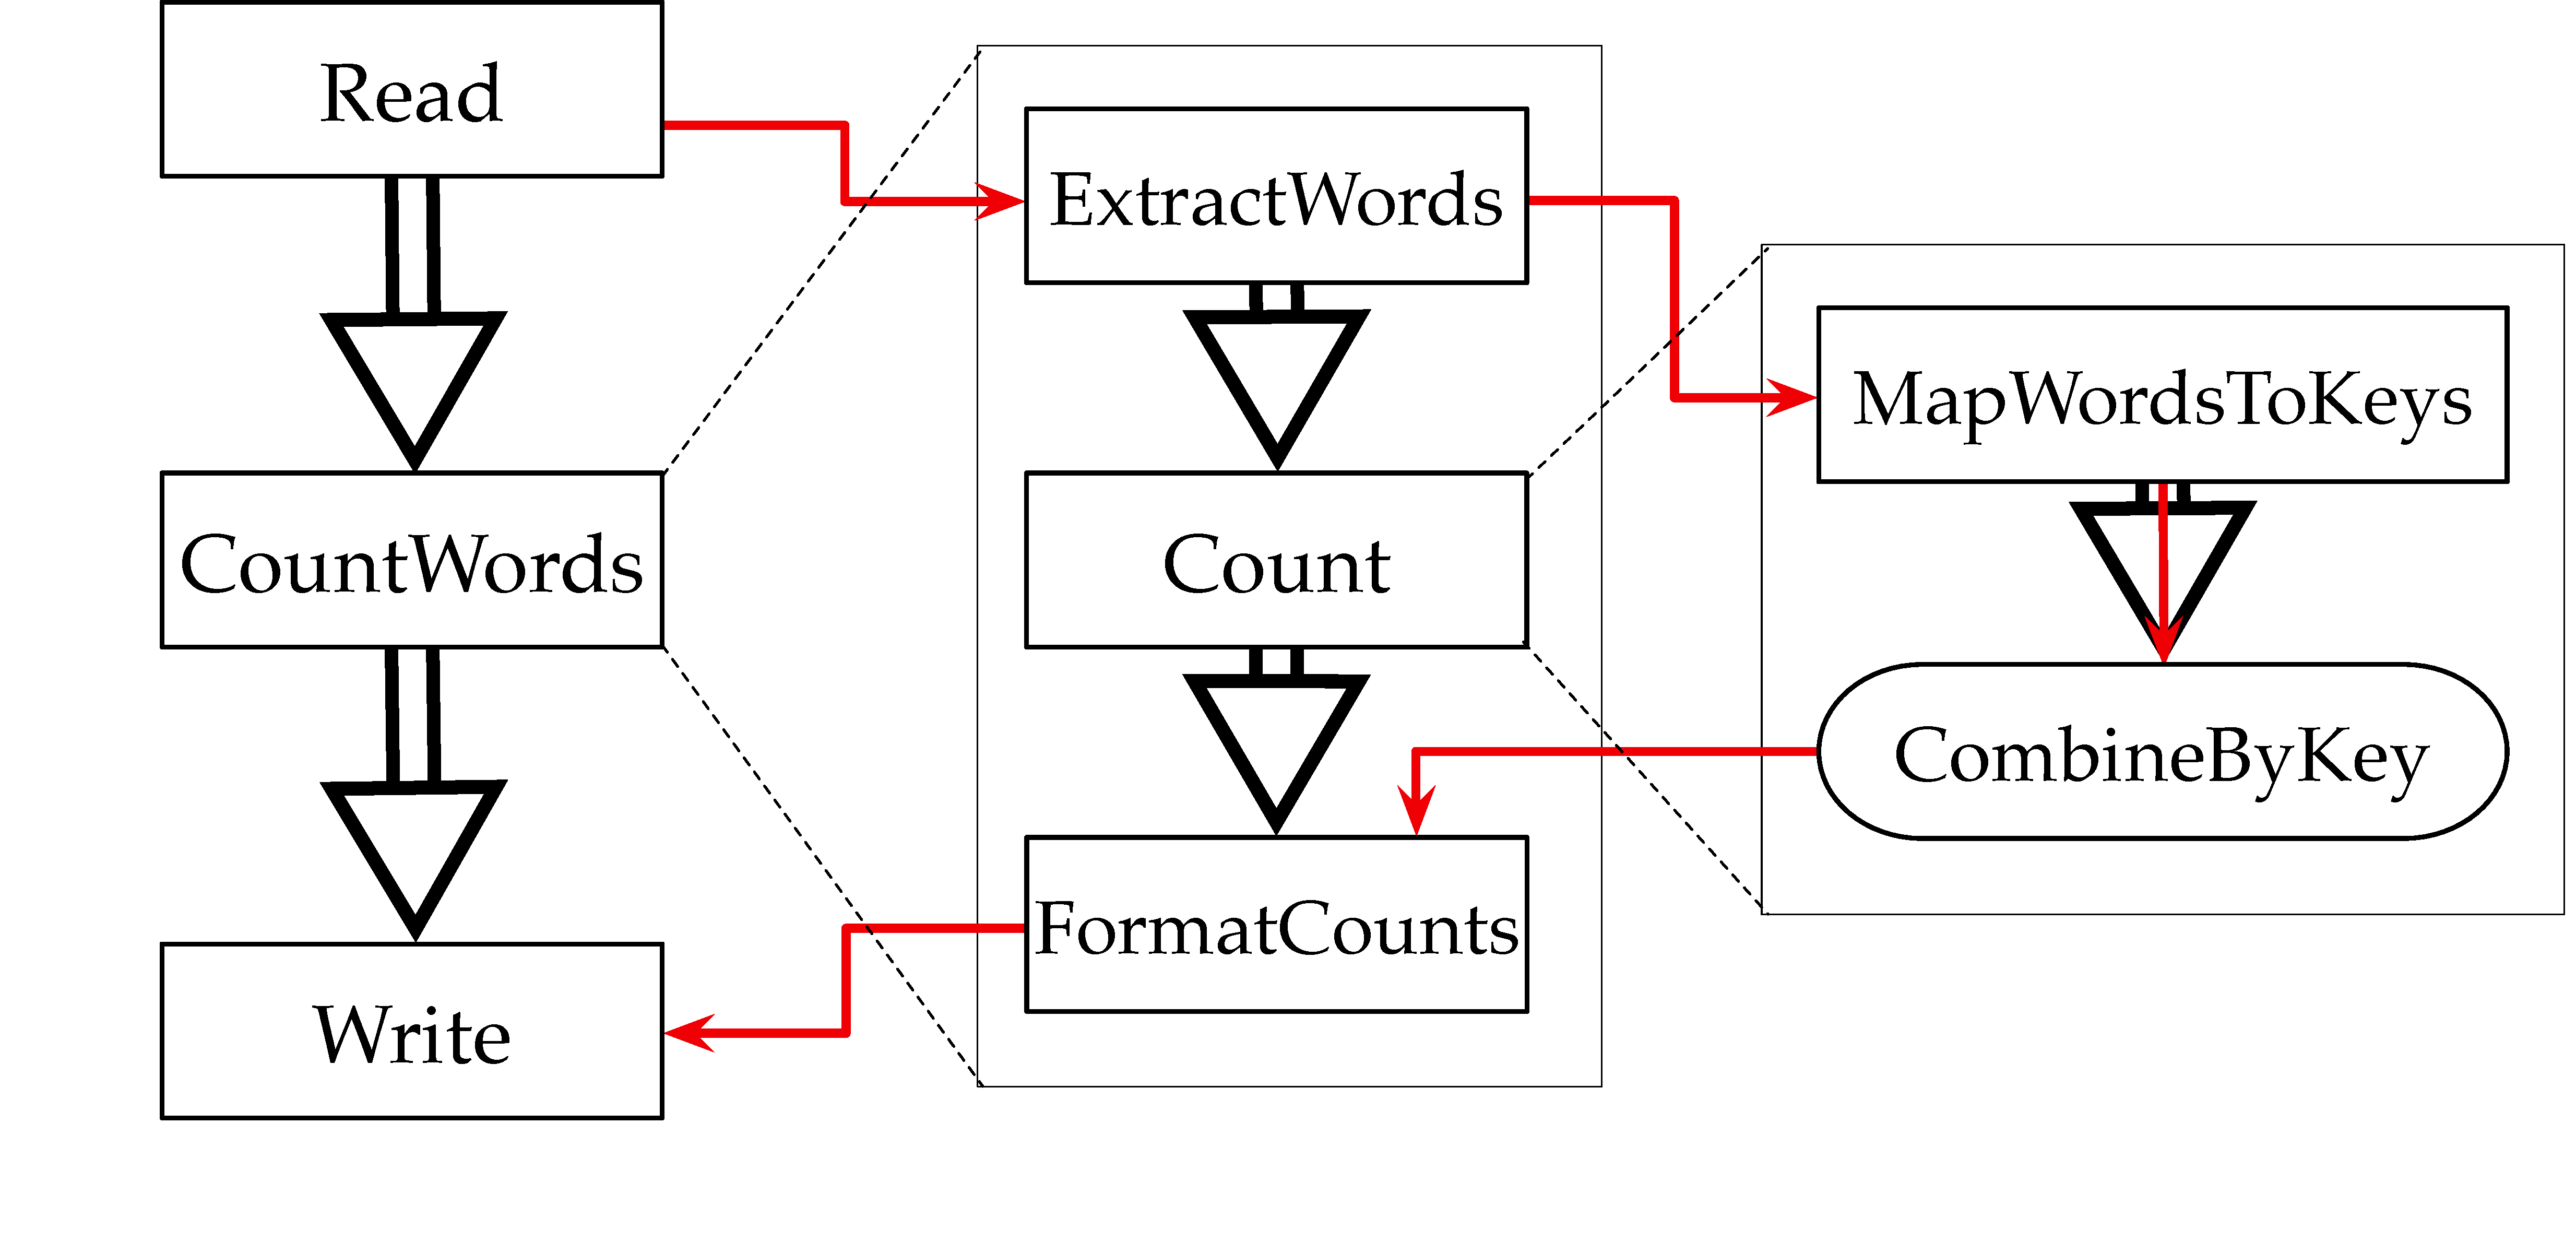
\includegraphics[width=\textwidth]{images/diags/composite-example}
	\caption[An illustration of the function of Composite Transforms in a typical Pipeline.]{A typical Pipeline uses Composite Transforms. The large arrows indicate the conceptual data flow path. The user expects to see visualisations or statistics using this abstraction. The thin red edges indicate the actual execution-time data flow---only leaf Transforms are instantiated and exchange data.}
	\label{fig:impl:composite-transforms}
\end{figure}

Each node in this graph is a \emph{Transform}.
Transforms can have multiple inputs or outputs.

Each edge in the graph represents a \emph{Collection}.
It is a description of the data that will be produced by a particular Transform.
Pipelines are constructed by \emph{applying} Transforms to Collections, resulting in new Collections which encode various information about the data, including the \emph{windowing strategy} the Collection will adopt and its producer.

Data is \emph{added} to a Collection whenever its producing Transform outputs data.
What this means in practice is implementation-dependent---Beam tracks Collections explicitly while the Elixir implementation uses them only to connect Transforms, after which they exchange data directly.

Transforms may be \emph{Primitive} or \emph{Composite}.
A Primitive Transform is directly executed by the Pipeline runner, while a Composite Transform \emph{expands} into multiple sub-Transforms (\cref{fig:impl:composite-transforms}).
Different runners may choose to implement different Transforms as primitives and provide composite implementations for the rest.

Composite Transforms are tracked for informational purposes (statistics, logging or visualisation), but don't actually get instantiated at execution-time.

As a side effect of the application of a Transform to a Collection, a node representing a particular instance of the Transform is added to the DAG.
Such a node is called an \emph{Applied~Transform}.
As well as the parameters of the Transform which was applied, it holds extra information used at execution-time.

When the Pipeline is executed, this Applied Transform will be instantiated into some runtime structure which is responsible for actually performing computation.
This may be an object in the case of Java or an actor process in the case of Elixir and is called a \emph{Transform~Executor}.

\subsection{Windows and panes}\label{sec:impl:dataflow:windows-panes}

As described in \cref{sec:prep:dataflow:where}, \emph{windows} are used to group elements in event-time (i.e.\ with regards to their intrinsic timestamps).
In practice, a window is a meta-value acting as a second key by which elements are grouped, usually taking the form of a time interval.

Transforms generally fall into two classes---\emph{Elementwise Transforms} and \emph{Grouping Transforms}.
These roughly correspond to the \verb|ParDo| / \verb|GroupByKey| distinction made in \cref{sec:prep:dataflow:what}.

Elementwise Transforms are essentially flat-map operations---they take input elements and for each one immediately output zero or more other elements.
Examples include \verb|Map|, \verb|FlatMap| and \verb|WindowInto|.

Grouping Transforms perform all operations partitioned by key and window.
They do not output any elements until they are triggered (described later).
Much of the core complex logic of the Model deals with Grouping Transforms and ensuring they produce correct data at the correct time.
Implementations make this behaviour available as a standard module or class to be used in such Transforms.

A \emph{pane} is an element produced by a Grouping Transform when a trigger fires, representing the output of that Transform for a given key and window.
It generally takes the form of a key-value pair.
For example, a \verb|GroupByKey| will output panes consisting of a key and a list of values which had that key and were in the given window.

\subsection{Watermarks and lateness}\label{sec:impl:dataflow:watermarks}\label{sec:impl:dataflow:lateness}

As mentioned in \cref{sec:prep:dataflow:when}, a \emph{watermark} is a heuristic indicating progress in the event stream.

Theoretically, each Collection has its own true watermark.
In practice, this is not knowable or even sometimes computable, and so \emph{local watermarks} are used.

\begin{figure}[t]
	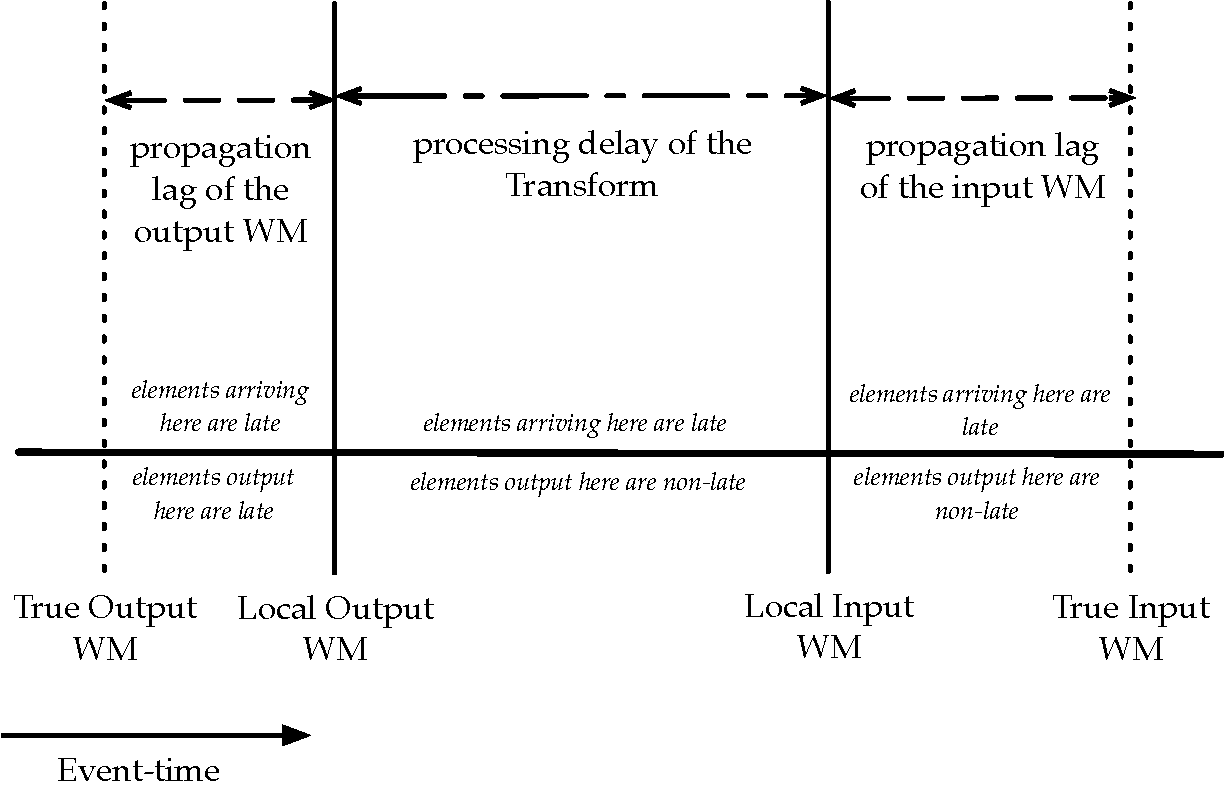
\includegraphics[width=\textwidth]{images/diags/lwm-transform-instantaneous}
	\caption{The watermarks of a Transform at a single point in processing-time.}
	\label{fig:impl:lwm-instantaneous}
\end{figure}

Each Transform has \emph{local input (LIWM)} and \emph{output (LOWM) watermarks}, illustrated in \cref{fig:impl:lwm-instantaneous}.
A LIWM is a lower bound on the true watermarks of all input Collections, and a LOWM is an upper bound on the true watermarks of all output Collections.

Reading the LIWM informs the Transform that no elements earlier than that time will arrive.
Likewise, when a Transform publishes a LOWM, it is indicating that it will not output any elements timestamped before that time. This induces an intuitive intuition of \emph{doneness}: a Transform is \emph{done} when its output watermark advances to infinity (since this implies that it will never produce any elements again).

All watermarks are monotonically increasing.
Further, it is required that (for ordinary Transforms) the LOWM does not advance beyond the LIWM.
In general, elements retain their timestamp on transformation.
Allowing the LOWM to overtake the LIWM could place the Transform in a state where a non-late (abiding by the watermark) input element causes output which would be late (behind the watermark) if emitted.

The above situation would violate a fundamental invariant of the system which is crucial to its design and allows us to reason about the computation in the face of unbounded, unordered data:

\textbf{Only late input can result in lateness anywhere in the system.}

\subsubsection{Lateness}

An element added to a Collection is \emph{late} if its timestamp is less than the true watermark of the Collection at the time of addition, and \emph{non-late} otherwise.

This definition uses the true watermark of a Collection.
To apply it in practice, the correspondence between an element's position with respect to a Transform's local watermarks and its lateness---as defined above---must be clarified.
\Cref{fig:impl:lateness-knowability} summarises this at a high level.

\begin{figure}[t]
	\subfloat[][The knowability of the lateness of an input element with respect to the LIWM.]{
		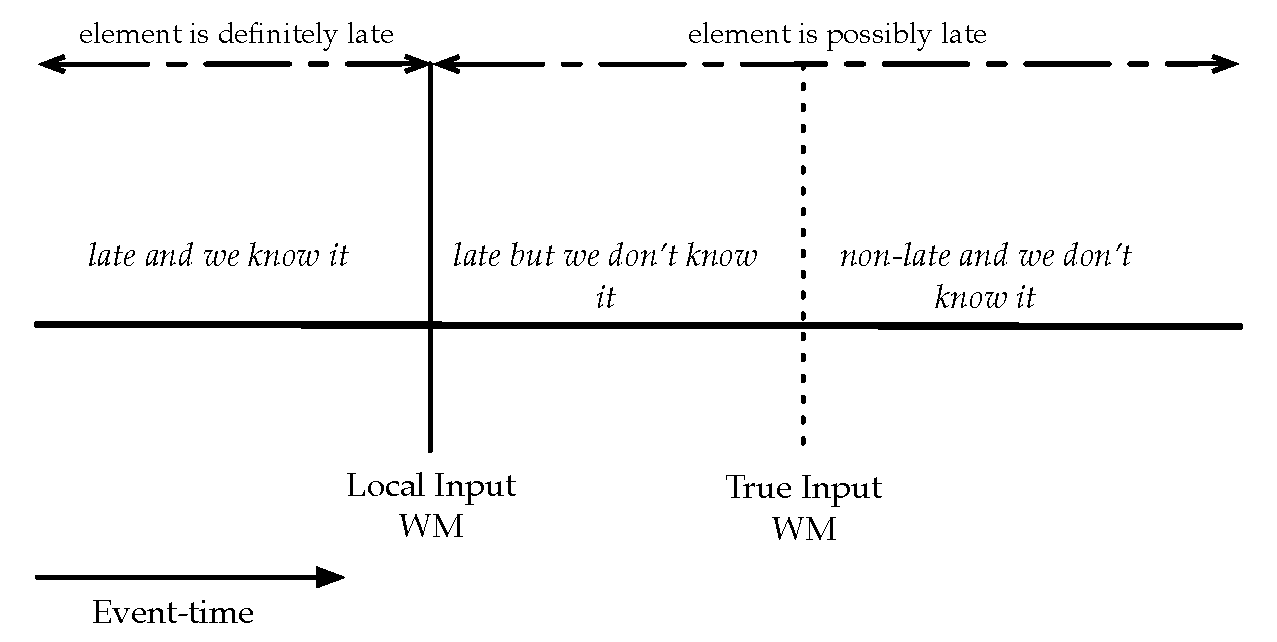
\includegraphics[width=\textwidth]{images/diags/lateness-knowability-input}
	}\\
	\subfloat[][The knowability of the lateness of an output element with respect to the LOWM.]{
		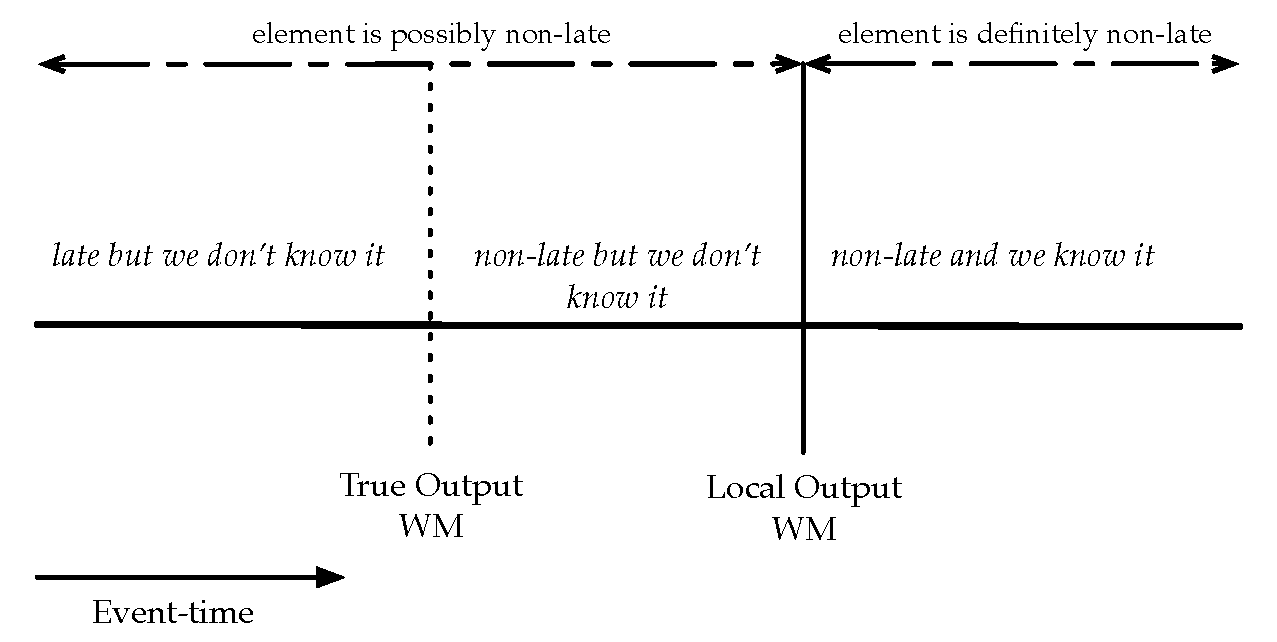
\includegraphics[width=\textwidth]{images/diags/lateness-knowability-output}
	}
	\caption{The lateness of elements with respect to local watermarks can only approximate their lateness with respect to the true watermark.}
	\label{fig:impl:lateness-knowability}
\end{figure}

It is clear that an algorithm must be devised which can deal with incomplete information about the lateness of elements.
For late elements, it must also decide whether they are late enough to be dropped silently.
Further, it must take into account user choices about the strategies to employ and compute the proper labelling of panes as they are output.
Throughout this, the issue of windows merging at arbitrary times must also be considered.

These issues are resolved through exhaustive case analysis described in detail by Knowles and Shields in an Apache Beam proposal~\cite{BEAM-doc-lateness}.
The algorithm described therein is implemented both in Beam and in Elixir Dataflow.
A high-level overview of the decisions made in its design is presented below.

\subsubsection{Grouping Transform algorithm}

The goal of the system is to avoid lateness where possible, without holding back Pipeline progress.
This means that data which is late at one stage of the Pipeline can be integrated into an output pane which is non-late at the next---perhaps taking advantage of the slower processing speed of the latter stage.
However, progress cannot be held back intentionally in order to accommodate this process.
These goals govern the resolution of the uncertainty in \cref{fig:impl:lateness-knowability}, generally erring on the side of treating elements as non-late.

Some requirements are also made of panes.
For a particular window (per-key), only one \verb|ON_TIME| pane can be output.
All \verb|EARLY| panes must be output before it, and all \verb|LATE| panes after it.
Panes are elements in themselves, and as such have their own timestamp (derived from the timestamps of their source elements).
It is required that \verb|EARLY| and \verb|ON_TIME| panes be non-late (when viewed as elements).

We say an element is \emph{on-time} if it is both deemed to be non-late and it arrives in time to be incorporated into an \verb|ON_TIME| pane.
The \verb|ON_TIME| pane cannot be output until the watermark has passed the end of the window---in this way, it is certain that all elements which are actually non-late will be included in this pane, as well as any `lucky' late elements.
This additionally implies that any \verb|LATE| pane is derived exclusively from late input elements.

\subsubsection{Watermark holds}

By default, a Transform's output watermark will be equivalent to its input watermark less a processing delay.
A Grouping Transform, however, must satisfy the invariants described above.
For instance, it must ensure that certain panes are output non-late.
Due to a flexible triggering model, output may not necessarily be synchronised with the input watermark.
At the same time, it is undesirable to write bespoke watermark-management logic for each Transform separately.

Instead, a Transform can specify a \emph{watermark hold} per-window-per-key.
The output watermark will then be the minimum of the input watermark and the earliest watermark hold set.
When a pane is output for a particular key and window, its associated hold is cleared, allowing the watermark to advance.

Additional care is needed to ensure that a hold is never placed after it is meant to be cleared, stopping progress.
An algorithm to ensure this, originating in Beam~\cite{BEAM-code-WatermarkManager}, is summarised in the appendix~(\cref{apx:additional:watermark-holds}).

\subsection{Triggers and timers}\label{sec:impl:dataflow:triggers-timers}

\emph{Triggers} (introduced in \cref{sec:prep:dataflow:when}) describe when output should be produced by a Grouping Transform.
This section gives an overview of their semantics and implementation.

\subsubsection{Triggers as state machines}
Triggers can be thought of as Finite State Machines (FSMs); indeed, the Beam implementation places its trigger logic in classes extending \verb|TriggerStateMachine|.

A Trigger FSM is instantiated per-window-per-key and is used by the Transform to make decisions on when to output.
A Trigger \emph{fires} when it instructs the Transform to output a pane.
A Trigger firing is binary---if it fires, all currently accumulated data is output into a pane, which is timestamped and marked appropriately.

The overall behaviour of the FSM is best showcased by looking at the \exs{TriggerDriver} behaviour\footnote{An Elixir \emph{behaviour} is a contract for a module to implement. An implementing module can then be chosen or provided at runtime and its functions (with signatures conforming to the behaviour) called dynamically by another module~\cite[281]{Thomas:2016}.} in Elixir Dataflow ~(\cref{lst:impl:trigger_driver}).

\begin{listing}[h]
	\begin{minted}{elixir}
defmodule Dataflow.DirectRunner.ReducingEvaluator.TriggerDriver do
  alias Dataflow.Utils.Time
  alias Dataflow.{Trigger, Window}
  
  @opaque state :: any
  
  # `timing_manager` is the pid of the Transform's TimingManager.
  # It allows the TriggerDriver to set and clear timers asynchronously
  # as well as reading watermark state
  @callback init(Trigger.t, Window.t, timing_manager :: pid) :: state
  @callback process_element(state, Time.timestamp) :: state
  @callback merge([state], state) :: state
  @callback should_fire?(state) :: boolean
  @callback fired(state) :: state
  @callback finished?(state) :: boolean
end
	\end{minted}
\caption[The \exs{TriggerDriver} behaviour showing the Finite State Machine design of a Trigger.]{The \exs{TriggerDriver} behaviour shows the FSM design of a Trigger. The functional paradigm of Elixir allows for the clean specification of the semantics as a set of transformations on state.}
\label{lst:impl:trigger_driver}
\end{listing}

The module's \exs{init} function is called to obtain the Trigger's initial state.
A series of \exs{process_element} calls then occurs, allowing the Trigger to update its state based on timestamps of incoming elements.
During any of these calls, the Trigger can also query the watermark positions in order to compute its next state.
The module may also be asked to \exs{merge} together states for several windows into a new state for the resultant window.

The Trigger itself does not asynchronously notify the Transform of its firing.
Instead, the Transform will query the Trigger to check if it should fire using \exs{should_fire?}.
These queries will be the result of timers set by the Trigger.
If the Trigger fires, a pane of output is produced (according to the rules in \cref{sec:impl:dataflow:windows-panes}) and the Trigger is notified via the \exs{fired} callback.

A Trigger is \emph{closed} or \emph{finished} if it will never fire again.
The Trigger can be asked if it is finished using the \exs{finished?} callback.
At that point it is safe to remove the state associated with the entire window, leaving only a tombstone indicating that new elements in this window should be ignored.

The referentially transparent FSM pattern provides great flexibility in specifying triggering behaviour, but keeps the interface to this logic very simple.
It also allows Triggers to be composed into trees, as the Trigger acts identically whether it is queried by a Transform or a parent Trigger.
An example of this pattern is the \verb|AndThen| Trigger, which delegates to one Trigger until it is closed, switching to the second at that point.

The default Trigger used when no other Trigger is explicitly specified fires once when the input watermark passes the end-of-window, and fires again every time a late element is seen (producing a one-element \verb|LATE| pane).
The implementation of this default Trigger in Elixir can be found in \cref{lst:apx:additional:default-trigger} in the appendix.

\subsubsection{Timers}

\emph{Timers} are used to schedule an asynchronous notification in the future.
A \emph{timer} is a tuple of \exs{{namespace, time, domain}}\footnotemark, with the \exs{domain} being one of processing-time or event-time.

\footnotetext
{
In Beam, timers also have a unique ID, used to identify and compare them. This is not needed in Elixir, since they can be directly compared as values.
}

Once a timer is set, the Transform will receive an asynchronous notification when it fires.
This will happen when the input watermark (event-time) or clock time (processing-time) passes the \exs{time} of the timer.
Multiple timers may fire simultaneously, and the Transform Executor will be notified of all of them.

The \exs{namespace} of a timer is an arbitrary value, but in practice is used to associate timers to the Triggers that set them, or to keep track of different timers in specialised Transforms.
Often, the namespace is not even used in a timer handling callback (all timers are treated the same), but rather only employed to clear specific timers before they fire.

No semantics are implied by the timers themselves---they merely provide a mechanism to receive a notification with a particular identifier at a particular time.
It is up to the Transform to interpret this and act accordingly---for example by asking its Trigger whether it is ready to fire.

\subsection{Watermark generation and processing}\label{sec:impl:dataflow:watermark-generation}

Previous sections address the preservation of the correctness of watermarks and the non-lateness of elements as they pass through a Transform.
It remains unclear how a watermark is initially generated.

This process is crucial, as it is the only part of the system in which lateness can be introduced.
It also very application-specific.
For some data sources, we can get a guaranteed-correct read-position.
For others, the source provides us with only an approximation.
In yet other cases, statistics must be kept about the source to generate a heuristic.

There is no standard solution---a mechanism is needed to allow flexibility in watermark generation.
This is provided by \emph{Sources}---application-specific code which produces a watermarked Collection when used by a \verb|Read| Transform.

At execution, the \verb|Read| Transform will use logic found in the Source to assign timestamps to elements being read (e.g.\ Kafka message timestamps) and to publish a monotonically increasing watermark.
A Bounded Source with no intrinsic timestamps will generally output a minimal watermark (and timestamp all output with the minimal timestamp) until it is finished, advancing the watermark to the maximal timestamp to indicate that.

Sources for popular data sources such as the file system, Apache Kafka and Google BigQuery are included in Beam, and an API~\cite{BEAM-code-SourceAPI} is provided to add custom Sources (in fact, this API is used in \cref{sec:eval:twitter:code}).

\subsubsection{Watermark domains}

Limiting the generation of watermarks to Sources allows for encapsulation of potentially lateness-introducing code.
However, it can cause problems from a user perspective and limit the flexibility of the Model.
This problem has been discussed but unaddressed in Beam~\cite{Beam-JIRA-watermark-domains}.
However, this project implements a solution.

Suppose a Pipeline receives data containing names of log files in cloud storage.
These files contain log entries collected during a particular day, which are then dumped to storage during log rotation every 24 hours.
The timestamp of these elements will be the timestamp of the file, which will be \textbf{after} all of the entries in the file.

A Transform which outputs individual log entries given an input file will consistently output late data, as all entries in a log file will be older than the log file timestamp (which is used to generate the watermark in the Pipeline).
In fact, these new elements should not be considered late, because they belong in a different \emph{watermark domain} than the files containing them.

Collections are in the same watermark domain when their elements' timestamps directly relate to one another \textbf{independently of element data}.
For example, when extracting body text from a social post, it makes sense to assign the same timestamp to the text as was assigned to the post itself.
We don't need to actually look at the post to make that decision.
Similarly, a Grouping Transform treats data aggregation and timestamp aggregation orthogonally.

However, in the log-file example above, the timestamp of an individual log entry generated from a file will be dependent on the data of the log entry itself---the recorded time of its generation.
A guarantee such as `the timestamp of an entry will never be earlier than 24 hours before the timestamp of its file' may exist, but this again is an application-specific decision, unsuitable for inclusion in a generic model.

Such a guarantee constitutes a watermark.
This watermark, however, is not computed from the input watermark in a way consistent with the lateness invariants and rules in \cref{sec:impl:dataflow:lateness}.

This conflict is resolved by breaking the Pipeline into several watermark domains.
The invariants and relationships described earlier hold only within one watermark domain and not across them.

The lateness semantics only make sense when applied to data which can all be semantically described with one time domain.
At a domain boundary, there is no general solution to obtaining the correct watermark---the problem once-again becomes application-specific.
The problem is similar to that of ingesting data into a Pipeline, and it is solved similarly.

Certain Transforms can declare that they initiate a new watermark domain.
These Transforms may directly manage their own output watermark with no restrictions on its relation to the input watermark.

This, of course, introduces a potential source of lateness at every point such a Transform is placed in the Pipeline.
However this too is semantically valid.
At these points, timing information which did not exist in the Pipeline is extracted.
Since this information is unavailable at earlier stages, it is impossible for previous transformations to have taken account of it in determining whether input to the system was late.
Instead, its possible effect on the lateness of data is considered as soon as the information is actually known, with the lateness system carrying those effects downstream.

This solution also potentially simplifies the original approach to Sources by allowing for decoupling of logic.
An example of this can be seen in one of the Evaluation examples~(\cref{sec:eval:twitter:code}).

\section{The Dataflow DSL}\label{sec:impl:approach}\label{sec:impl:approach:dsl}

The design of a usable, intuitive Domain Specific Language (DSL) for constructing Pipelines was an important component of this project, and one of its original goals.

As described in \cref{sec:prep:elixir:basics}, Elixir encourages programmers to express computations as series of data transformations using the pipeline operator \exs{|>}.
Thus, the Dataflow approach to expressing computation translates naturally into Elixir with only a minimal amount of additional syntax.

\begin{listing}[h]
	\caption[An example of Pipeline construction in Elixir.]{An example of the construction and execution of a simple Pipeline in Elixir Dataflow.}
	\label{lst:impl:elixir-construct-pipeline}
	\begin{minted}{elixir}
use Dataflow
alias Dataflow.Transforms.{Core, IO, Aggregation}
alias Dataflow.DirectRunner

pipeline = Pipeline.new

pipeline
~> IO.read_file("data/data1.txt")
~> Aggregation.count_elements()
~> "Format Counts" -- Core.map(fn {word, count} -> "#{word}: #{count}" end)
~> IO.write_file("data/output.txt")

DirectRunner.run pipeline, sync: true

	\end{minted}
\end{listing}

\Cref{lst:impl:elixir-construct-pipeline} illustrates the API with a simple working example.
A file which contains a single word on each of its lines is read.
The number of occurrences of each word is counted, formatted as a string, and output to another file.
\Cref{fig:impl:dsl-simple-pipeline} shows this Pipeline as a DAG.

\begin{figure}[h]
	\centering
	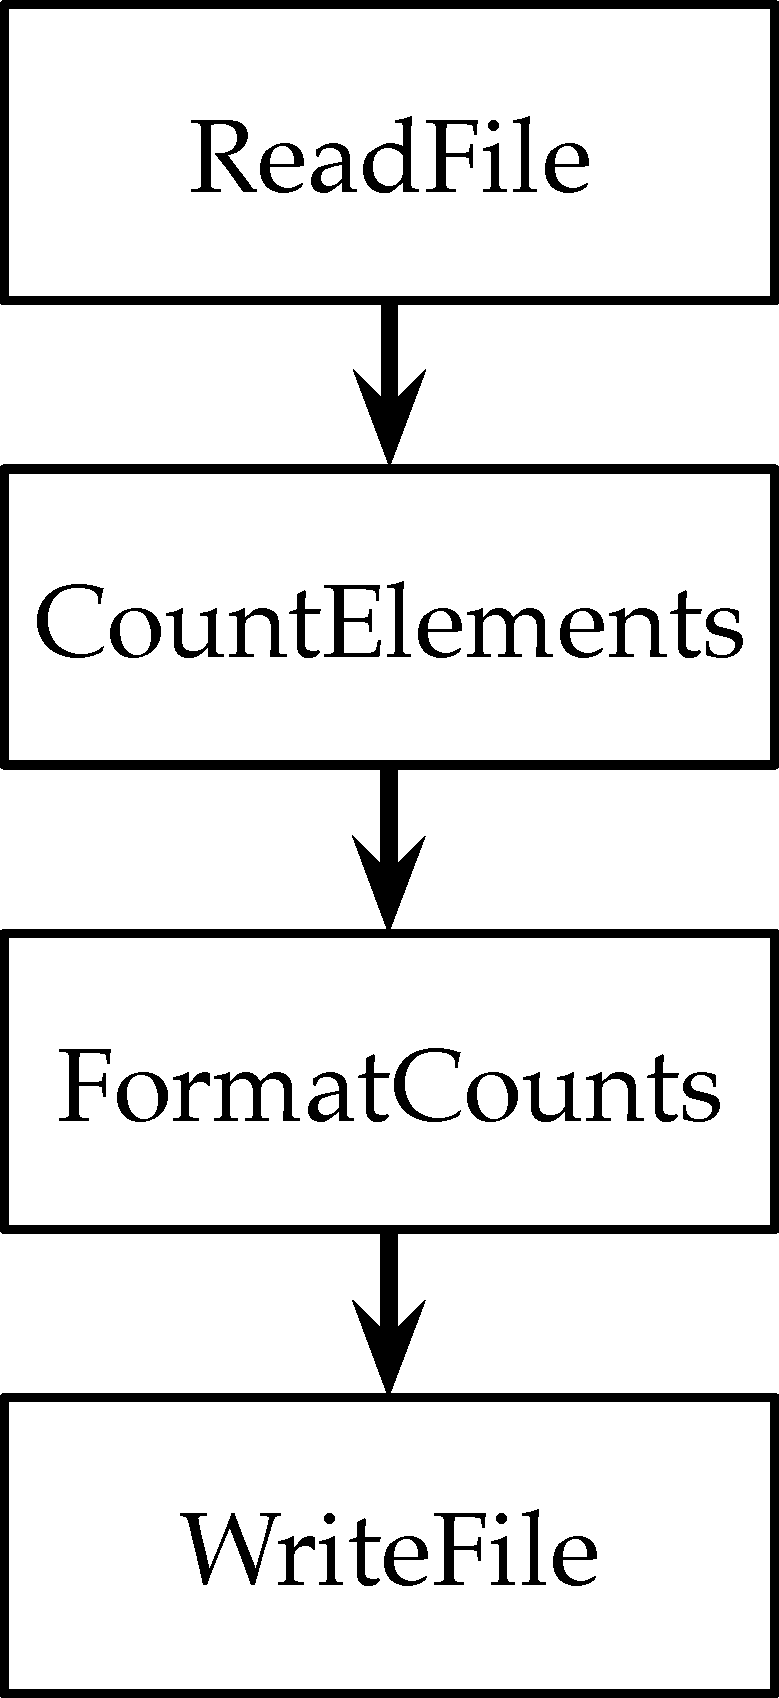
\includegraphics[width=0.2\textwidth]{images/diags/dsl-simple-pipeline}
	\caption[A simple Pipeline constructed in \cref{lst:impl:elixir-construct-pipeline}.]{\Cref{lst:impl:elixir-construct-pipeline} constructs this simple Pipeline.}
	\label{fig:impl:dsl-simple-pipeline}
\end{figure}

In line 10, the \exs{--} operator is used to assign a label to a particular Transform.
Assigning labels to Transforms is a feature useful for managing and visualising Pipelines.
This notation evokes the use of \verb|--| to denote a dash in \LaTeX.

\begin{listing}[h]
	\caption[An implementation of the computation in \cref{lst:impl:elixir-construct-pipeline} using standard sequential functions.]{The computation in \cref{lst:impl:elixir-construct-pipeline} can be expressed similarly using functions in the Elixir standard library.}
	\label{lst:impl:elixir-normal-comparison}
	\begin{minted}{elixir}
input = File.stream!("data/data1.txt")
output = File.stream!("data/output.txt", [:write])

input
|> count_elements() # local helper function
|> Enum.map(fn {word, count} -> "#{word}: #{count}" end)
|> Enum.into(output)
	\end{minted}
\end{listing}

\Cref{lst:impl:elixir-normal-comparison} shows an implementation of the same computation using Elixir standard library functions.
It demonstrates how closely the Dataflow Pipeline abstraction maps to existing paradigms in Elixir.

\subsection{Using macros}

In Elixir, \exs{--} is the list difference operator.
While it is possible to redefine the \exs{--} operator as one used for labelling Transforms, it would likely cause confusion.
Instead, Elixir macros enable this operator to take on a special meaning only in this particular context.

\emph{Macros} are powerful tools, allowing arbitrary AST transformation at compile-time~\cite[p.~13]{Elixir-Metaprogramming}.
The \exs{~>} operator is a macro.
Its definition~(\cref{lst:impl:elixir-dpipe-macro-def}) is short and delegates to a function right after parsing the special syntax.
This is a convention~\cite[p.~7]{Elixir-Metaprogramming} which ensures that macros do not end up causing unintuitive behaviour for the user.

\begin{listing}[h]
	\caption[The definition of the \exs{~>} macro for constructing Pipelines.]{The \exs{~>} macro is used to construct Pipelines. It transforms domain-specific syntax into simple function calls.}
	\label{lst:impl:elixir-dpipe-macro-def}
	\begin{minted}[autogobble]{elixir}
  defmacro pvalue ~> transform_with_label do
    case transform_with_label do
      # matches an `opts <> transform` AST node
      {:<>, _, [opts, transform]} ->
        quote bind_quoted: [pvalue: pvalue, transform: transform, opts: opts] do
          Dataflow.__apply_transform__(pvalue, transform, opts)
        end
        
      # matches a `label -- transform` AST node
      {:--, _, [label, transform]} ->
        quote bind_quoted: [pvalue: pvalue, transform: transform, label: label] do
          Dataflow.__apply_transform__(pvalue, transform, label: label)
        end
      
      # matches any other AST node
      transform ->
        quote bind_quoted: [pvalue: pvalue, transform: transform] do
          Dataflow.__apply_transform__(pvalue, transform, [])
        end
    end
  end
	\end{minted}
\end{listing}

Macros are compile-time functions which take the ASTs of their arguments and return an AST node with which the macro is replaced.

The \exs{~>} macro works by pattern-matching on the structure of the second argument, which can be an AST node of the form \exs{label -- transform} (line 10) or something else (line 16).
The \exs{options <> transform} syntax is also accepted, but is currently used only to pass additional options for testing purposes.

The macro returns a new AST node which is a call to the \exs{Dataflow.__apply_transform__} function containing Transform application logic.
Matching at the AST level means that \exs{--} can be redefined only within this context, without needing to shadow the original definition in the entire module.

The \exs{quote} macro allows for the construction of an AST node by writing normal Elixir syntax while specifying which variables from the macro's environment should be bound to the environment of the resultant AST node (the \exs{:bind_quoted} option).

The \exs{use Dataflow} line in \cref{lst:impl:elixir-construct-pipeline} imports the \exs{~>} macro implicitly.
In fact, a \exs{use Module} statement just calls the \exs{Module.__using__} macro~\cite[p.~35]{Elixir-Metaprogramming}.
This convention allows for boilerplate reduction without the issues caused by e.g.\ Ruby's monkey-patching.

The result of an application of the \exs{~>} operator is the \emph{Collection} produced by the applied Transform.
Branching Pipelines such as the one in \cref{fig:impl:dsl-branching-pipeline} can be created by applying multiple Transforms to one Collection.
This is shown in \cref{lst:impl:diverging-pipelines}.

In order to instantiate a Root Transform (e.g.\ \exs{IO.read_file}), it is applied to the Pipeline itself.

\begin{listing}[h]
	\caption[An example of creating branching Pipelines through application of multiple Transforms to one Collection.]{Branching Pipelines can be created by applying multiple Transforms to the same Collection.}
	\label{lst:impl:diverging-pipelines}
	\begin{minted}[autogobble]{elixir}
pipeline = Pipeline.new

words =
  pipeline
  ~> IO.read_file("data.txt")
  ~> extract_words()
  
# save words to file
words ~> IO.write_file("words.txt")

# also get the top words and write them to another file
words
~> get_top_words()
~> IO.write_file("top_words.txt")
	\end{minted}
\end{listing}

\begin{figure}[h]
	\centering
	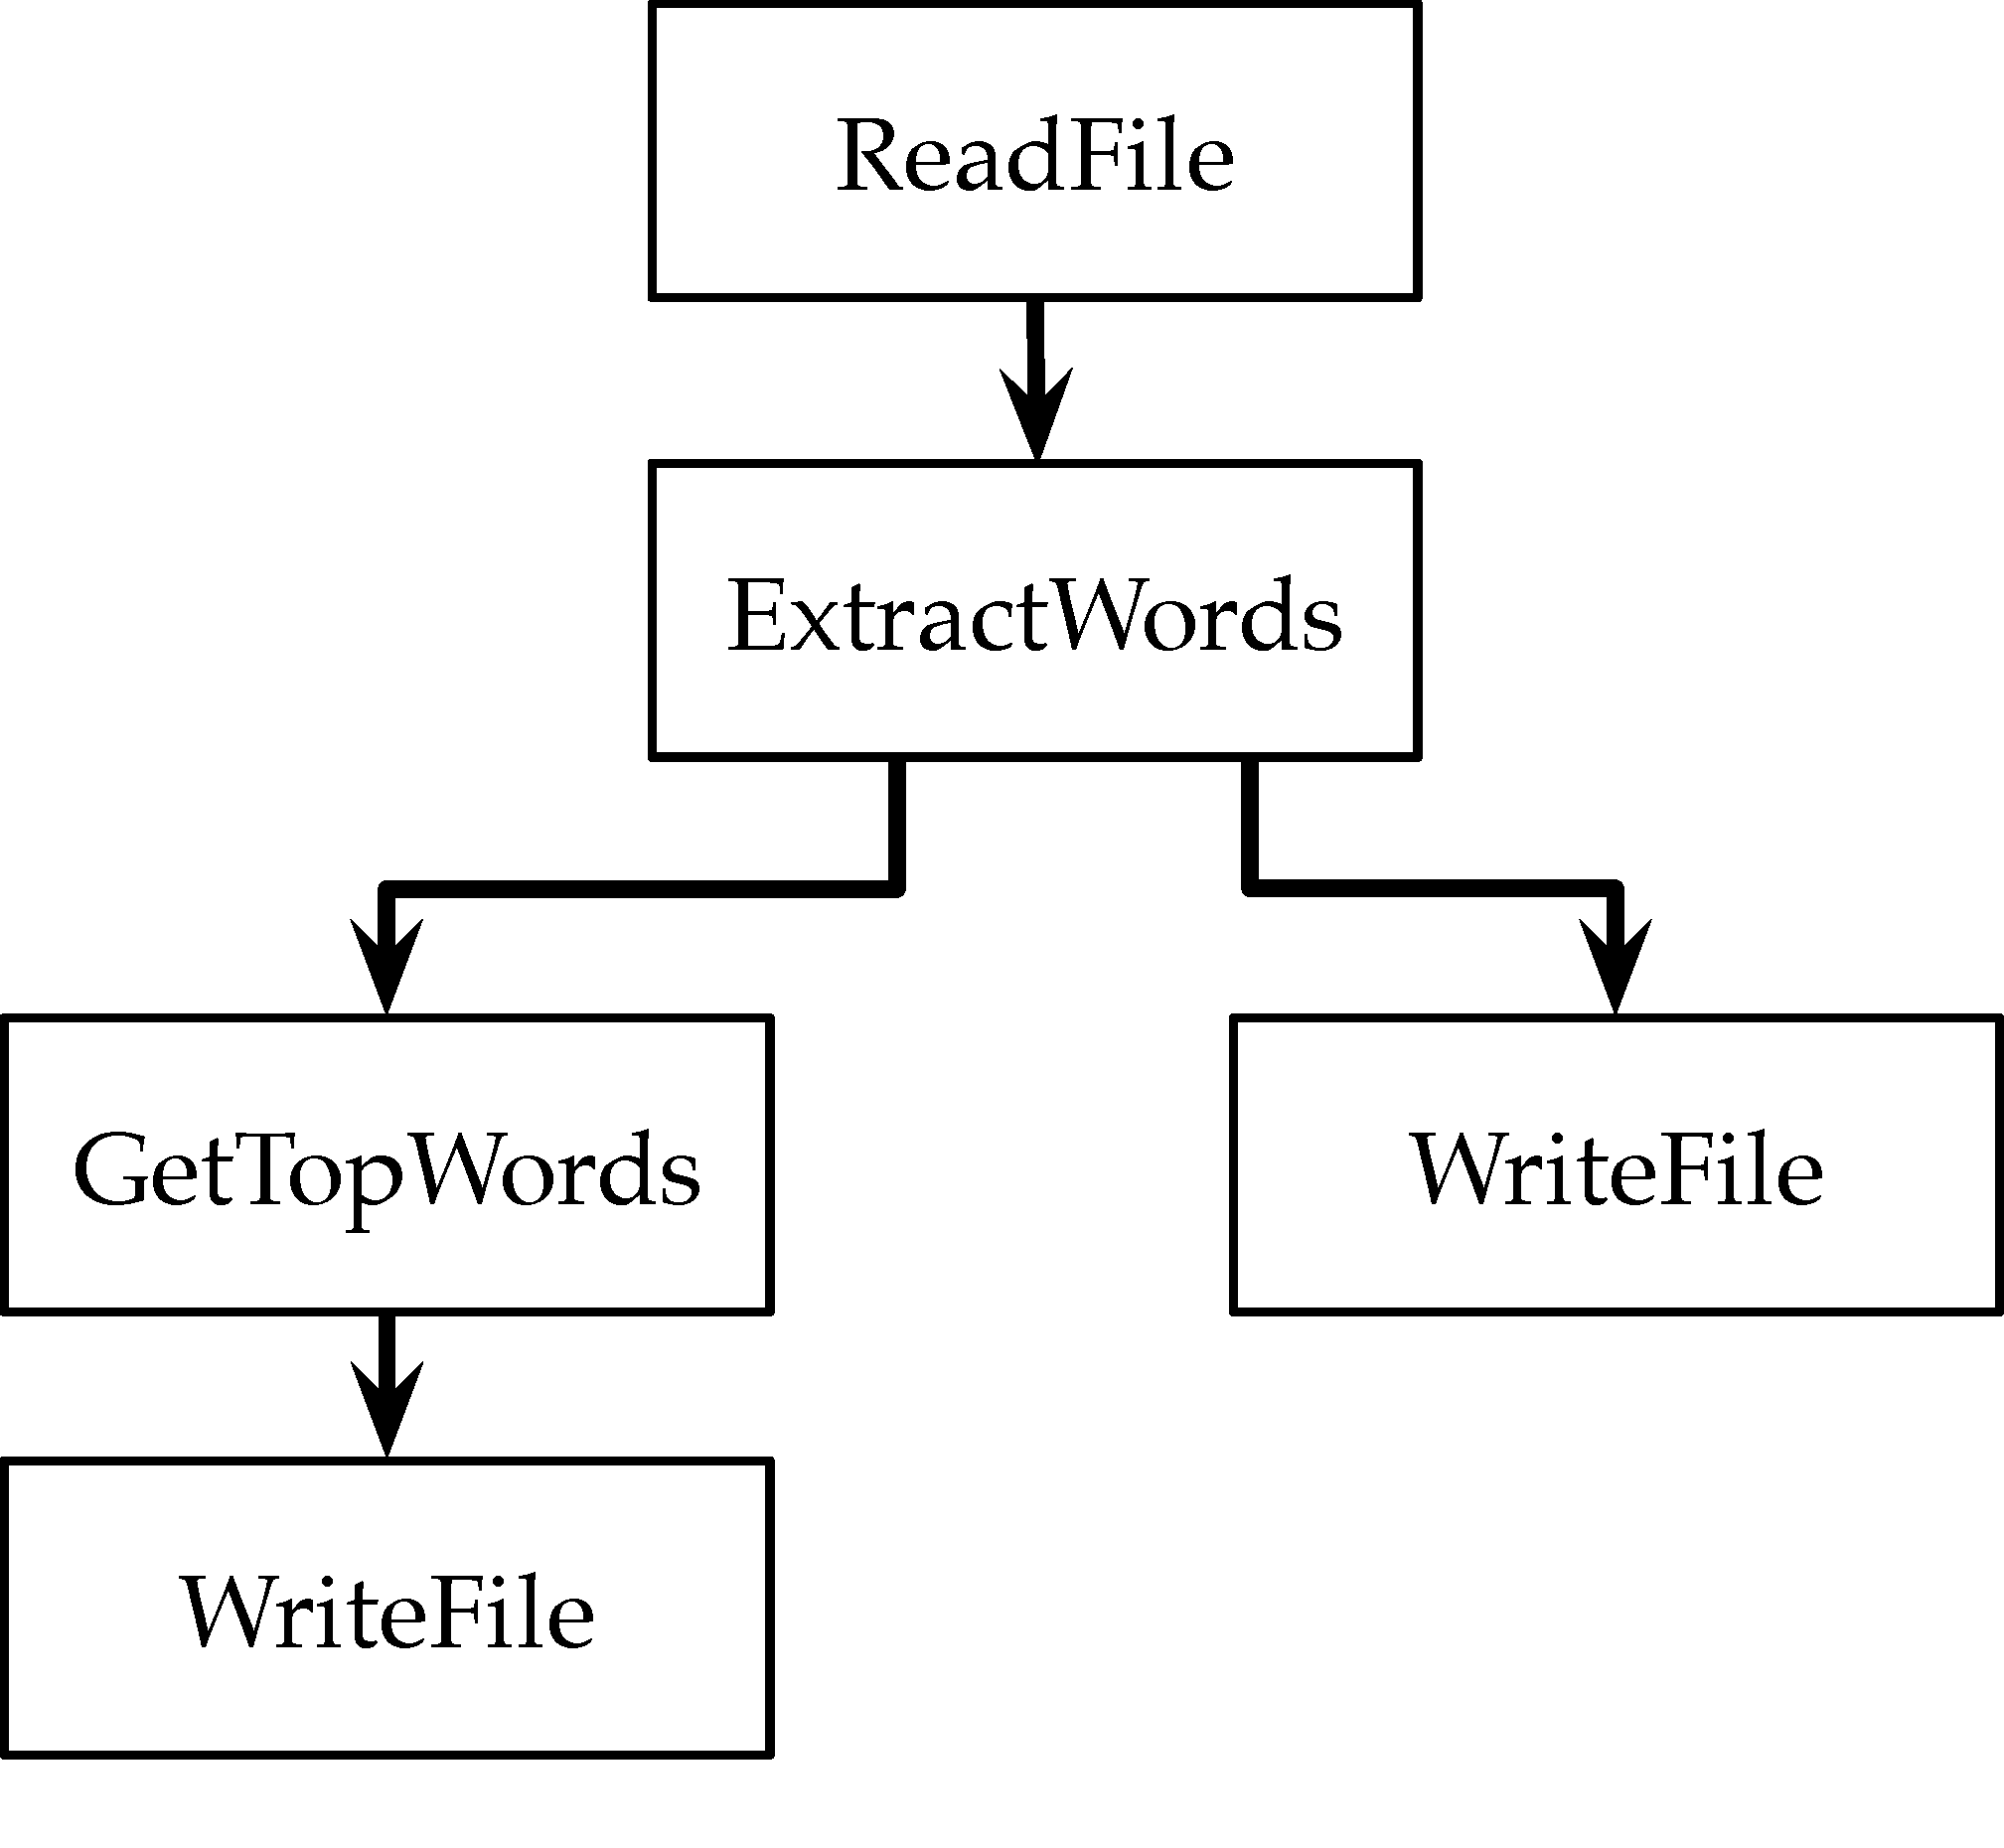
\includegraphics[width=0.6\textwidth]{images/diags/dsl-branching-pipeline}
	\caption[A branching Pipeline constructed in \cref{lst:impl:diverging-pipelines}.]{\Cref{lst:impl:diverging-pipelines} constructs a branching Pipeline---the result of \texttt{ExtractWords} is consumed by two other Transforms.}
	\label{fig:impl:dsl-branching-pipeline}
\end{figure}

\subsection{Structs and protocols}

Since there is a need to separate the construction and execution phases of the computation, a different approach is needed than in \cref{lst:impl:elixir-normal-comparison}, where on passing a value to a `transformation', the function is executed immediately.
Instead, the description of the computation must be stored in the Pipeline structure.

Elixir's protocols and structs are used in order to facilitate this.
A struct is a map with a \exs{:__struct__} key indicating its defining module.
It exhibits some special behaviour at compile-time, such as validation of key names.
A struct is always associated with a particular module.

A protocol is an interface module consisting of a set of function declarations.
Implementations of a protocol can then be defined on a per-module basis.
Protocol functions use dynamic dispatch to execute the correct implementation of the function given a struct argument.

\begin{sloppypar}
The functions in \cref{lst:impl:elixir-construct-pipeline}, such as \exs{IO.read_file}, don't perform any computation themselves---instead, they return a struct which stores their arguments and implements the \exs{PTransform.Callable} protocol.
For example, the result of calling \exs{IO.read_file("data.txt")} is \mintinline{elixir}{%IO.ReadFile{filename: "data.txt"}
}.
\end{sloppypar}

The definition of \exs{~>} in \cref{lst:impl:elixir-dpipe-macro-def} shows that these structs are subsequently incorporated into the Pipeline by calling a function which internally uses the protocol.

The definition of the Transform protocol is presented in \cref{lst:impl:ptransform-callable}.
The only requirement is for the Transform to be able to expand to more Transforms, behaving like Composite Transforms introduced in \cref{sec:impl:dataflow:pipelines-transforms-collections}.
Primitive Transforms are not definable by the user and receive special treatment, but the user is free to define their own Composite Transforms by providing an appropriate module and struct, much like one would define small, composable functions.

\begin{codelisting}
	\caption[The definition of the \exs{PTransform.Callable} protocol.]{The \exs{PTransform.Callable} protocol specifies that for a struct to describe a Transform, it must be able to \exs{expand} into sub-Transforms based on its input and parameters.}
	\label{lst:impl:ptransform-callable}
	\begin{minted}[autogobble]{elixir}
  defprotocol PTransform.Callable do
    # NestedState is a struct used on Pipeline construction to keep
    # track of Transform hierarchy.
    # User-defined Transforms can just treat it like a Collection.
    # 
    # a PValue is either a Collection, or a compound structure (e.g. tuple)
    # containing Collections.
    @spec expand(transform :: t, input :: Dataflow.Pipeline.NestedState.t)
            :: Dataflow.PValue.t
    def expand(transform, input)
  end
	\end{minted}
	
\end{codelisting}


\subsection{Managing DAGs using asynchronous processes}

Constructing and working with DAGs directly in a functional language is possible~\cite{Gibbons1995} but difficult, especially when advanced functional features such as those found in e.g.\ Haskell are not available.
Instead of attempting to do this, the concurrency model of Elixir was leveraged to simulate a mutable map of Collections and Applied Transforms inside the Pipeline structure.

The call to \exs{Pipeline.new} starts a new process which contains a map of the Collections (edges) and Applied Transforms (nodes) in the Pipeline graph, indexed by a unique integer ID.
This means that it is possible to arbitrarily add new structures to the DAG, even in the face of Composite Transforms or branching Pipelines.

\Cref{lst:impl:diverging-pipelines} shows that Pipelines behave like mutable objects---merely using the \exs{~>} operator on a Pipeline modifies it.
Therefore, Pipelines in this context are better thought of as processes rather than values.
However, once the construction of the Pipeline is finished, it is possible to freeze it and turn it into a simple data structure which once again behaves in the expected manner.
Indeed, the \exs{DirectRunner.run} function does this internally before taking this data structure and executing it.

